%% Preambulo, paquetes a cargar por compilador latex
\documentclass[12pt]{beamer}
\mode<presentation>{
  % selección de tema y color
  \usetheme{Copenhagen}
  \usecolortheme{orchid}
}

\usepackage[utf8]{inputenc}
\usepackage[spanish]{babel}
\usepackage{float}
\usepackage{graphicx}
\usepackage[font=scriptsize,labelfont=bf]{caption}
\usepackage{verbatim}
\usepackage{url} 
\usepackage[export]{adjustbox}
\usepackage{listings}
\usepackage{tcolorbox}
\usepackage{tikz}
\usepackage{cclicenses}
\usepackage{multicol}
\usepackage[autostyle]{csquotes}
\lstdefinestyle{mystyle}{
  basicstyle=\tiny,
  language=Python
}
\lstset{style=mystyle}

%% Automatizar localización de las imágenes
\graphicspath{{../img/}}

\title{Code Reviews con git avanzado}
\author[Pepe Doval]{Pepe Doval}
\institute[SetPay]{SetPay}
\date{\today}

\begin{document}

\begin{frame}
  \titlepage
  \begin{tcolorbox}[]
    \centering
    {\small \bysa}\\
    {\tiny Esta obra está suxeita á licencia
      Recoñecemento-CompartirIgual 4.0 Internacional de Creative
      Commons. Para ver unha copia desta licencia, visite
      http://creativecommons.org/licenses/by-sa/4.0/.}
  \end{tcolorbox}
\end{frame}

\begin{frame}
  \frametitle{Índice}
  \tableofcontents
\end{frame}

\usebackgroundtemplate{%
  \tikz[overlay,remember picture] 
  \node[opacity=0.3 , at=(current page.south east),anchor=south east] {
    
\includegraphics[]{logo-labs}};
}


\title[Code Reviews]{Code Reviews}
\date{}
\author[Pepe Doval]{}
\institute{}

\section{Code Reviews}
\label{sec:CodeReviews}

\usebackgroundtemplate{}
\begin{frame}
  \titlepage
\end{frame}

\usebackgroundtemplate{%
  \tikz[overlay,remember picture] 
  \node[opacity=0.3 , at=(current page.south east),anchor=south east] {
    
\includegraphics[]{logo-labs}};
}

\subsection{Introdución}
\label{subsec:Introducion}

\begin{frame}
  \frametitle{Canta xentiña!}
  \begin{figure}[ht]
    
\includegraphics[scale=0.18]{David_al_microfono}
  \end{figure}
\end{frame}

\begin{frame}
  \frametitle{Son un mal programador}
  \begin{figure}[ht]
    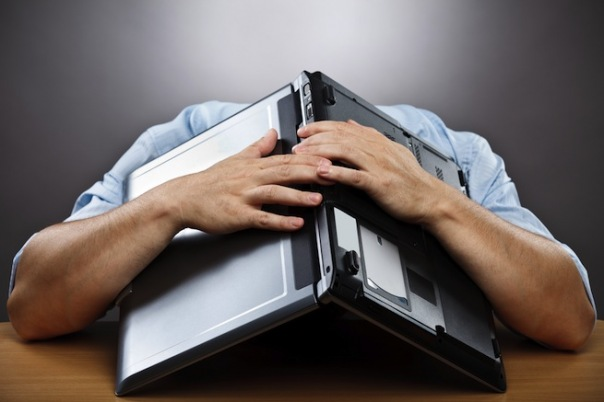
\includegraphics[scale=0.4]{sad_developer}
    \caption{http://csgardner.com/blog/2015/06/11/managing-software-developers/}
  \end{figure}
\end{frame}

\begin{frame}
  \frametitle{Pero tamén fun un crack}
  \begin{figure}[ht]
    
\includegraphics[scale=0.4]{zen_developer}
    \caption{https://www.apico.net/blog/how-bad-software-developer-are-you.html}
  \end{figure}
\end{frame}

\begin{frame}
  \frametitle{...é dicir, fun Junior}
  \begin{figure}[ht]
    
\includegraphics[scale=0.4]{happy_monkey}
    \caption{https://www.apico.net/blog/how-bad-software-developer-are-you.html}
  \end{figure}
\end{frame}

\begin{frame}
  \frametitle{De que vai construír software}
  \begin{figure}[ht]
    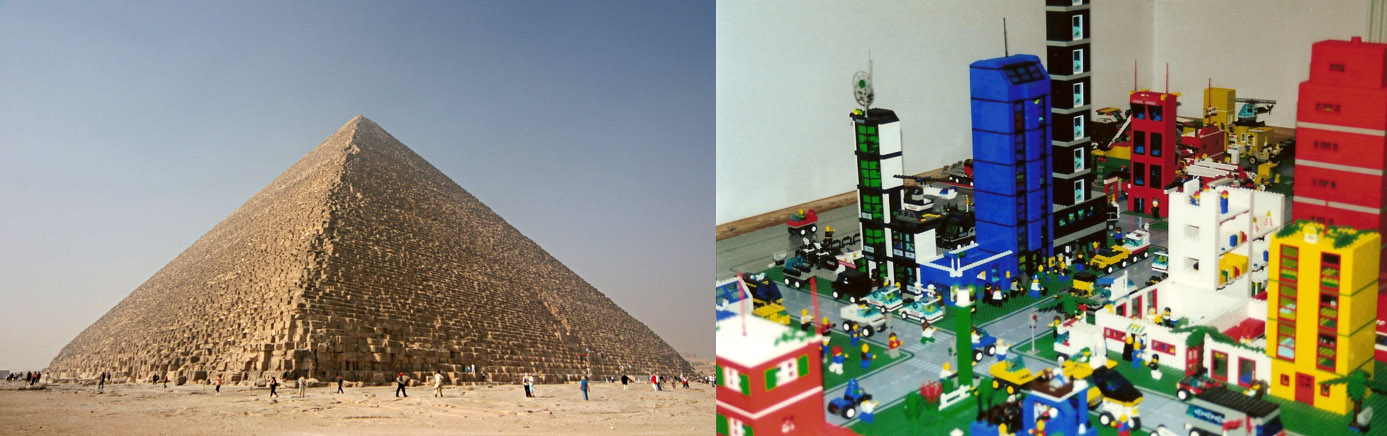
\includegraphics[scale=0.2]{pyramid_vs_lego}
    \caption{Wikipedia}
  \end{figure}
\end{frame}

\begin{frame}
  \frametitle{Abracemos o cambio}
    \centering
    O que hoxe está ben, mañá estará mal.
    \begin{figure}[ht]
      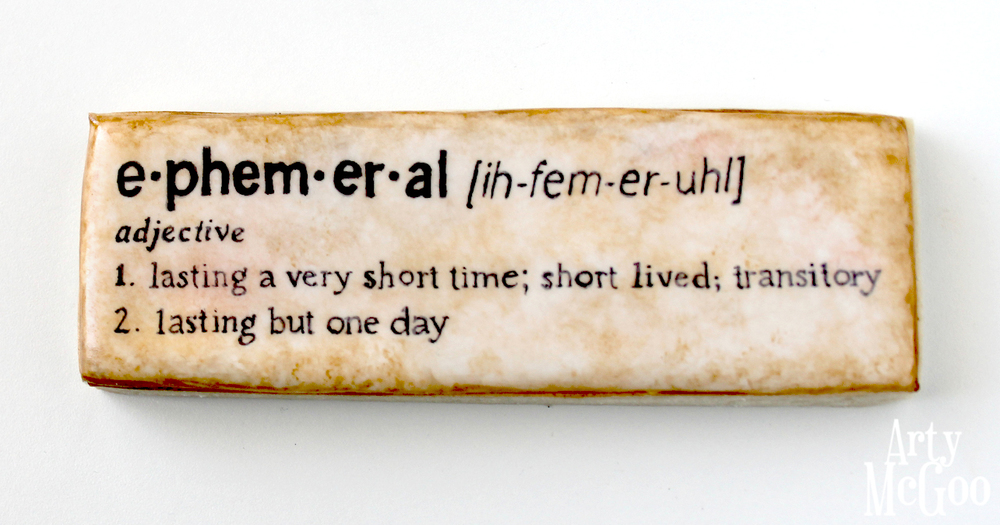
\includegraphics[scale=0.2]{ephemeral}
      \caption{http://www.artymcgoo.com/blog/2014/5/15/ephemeral-art}
    \end{figure}
\end{frame}

\begin{frame}
  \frametitle{Por que revisar código}
  \begin{itemize}
  \item Atopar erros
  \item Mellorar o código
  \item Compartir coñecemento
  \item Compartir decisións
  \item Mellorar a comunicación do equipo
  \end{itemize}
\end{frame}

\begin{frame}
  \frametitle{Mars Climate Orbiter}
  \begin{figure}[ht]
    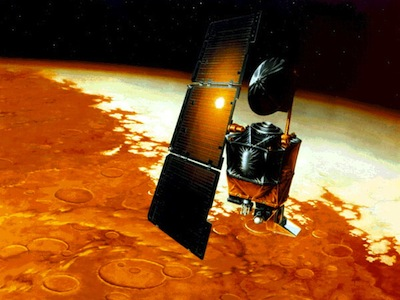
\includegraphics[scale=0.5]{mars_climate_orbiter}
    \caption{http://visionlearningcommunity.blogspot.com/2012/09/tragedies-in-science-crash-of-mars.html}
  \end{figure}
\end{frame}

\begin{frame}
  \frametitle{O día que non comezou a Terceira Guerra Mundial}
  \begin{figure}[ht]
    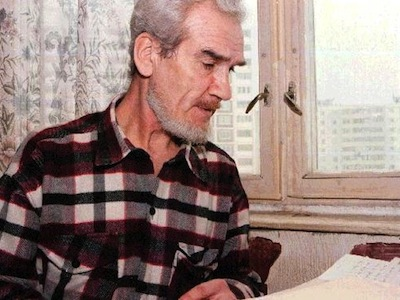
\includegraphics[scale=0.5]{petrov}
    \caption{http://www.brightstarsound.com/world\_hero/petrov\_expanded\_photo.html}
  \end{figure}
\end{frame}

\begin{frame}
  \frametitle{Se non queredes revisar código...}
  \begin{figure}[ht]
    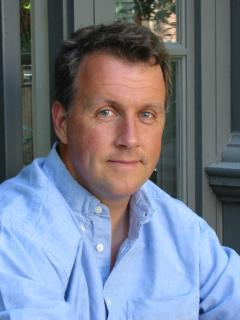
\includegraphics[scale=0.5]{Graham}
    \caption{Wikipedia}
  \end{figure}
\end{frame}

\subsection{Que é unha Code Review}
\label{subsec:Que}

\begin{frame}
  \frametitle{Que é unha Code Review}
  \begin{figure}[ht]
    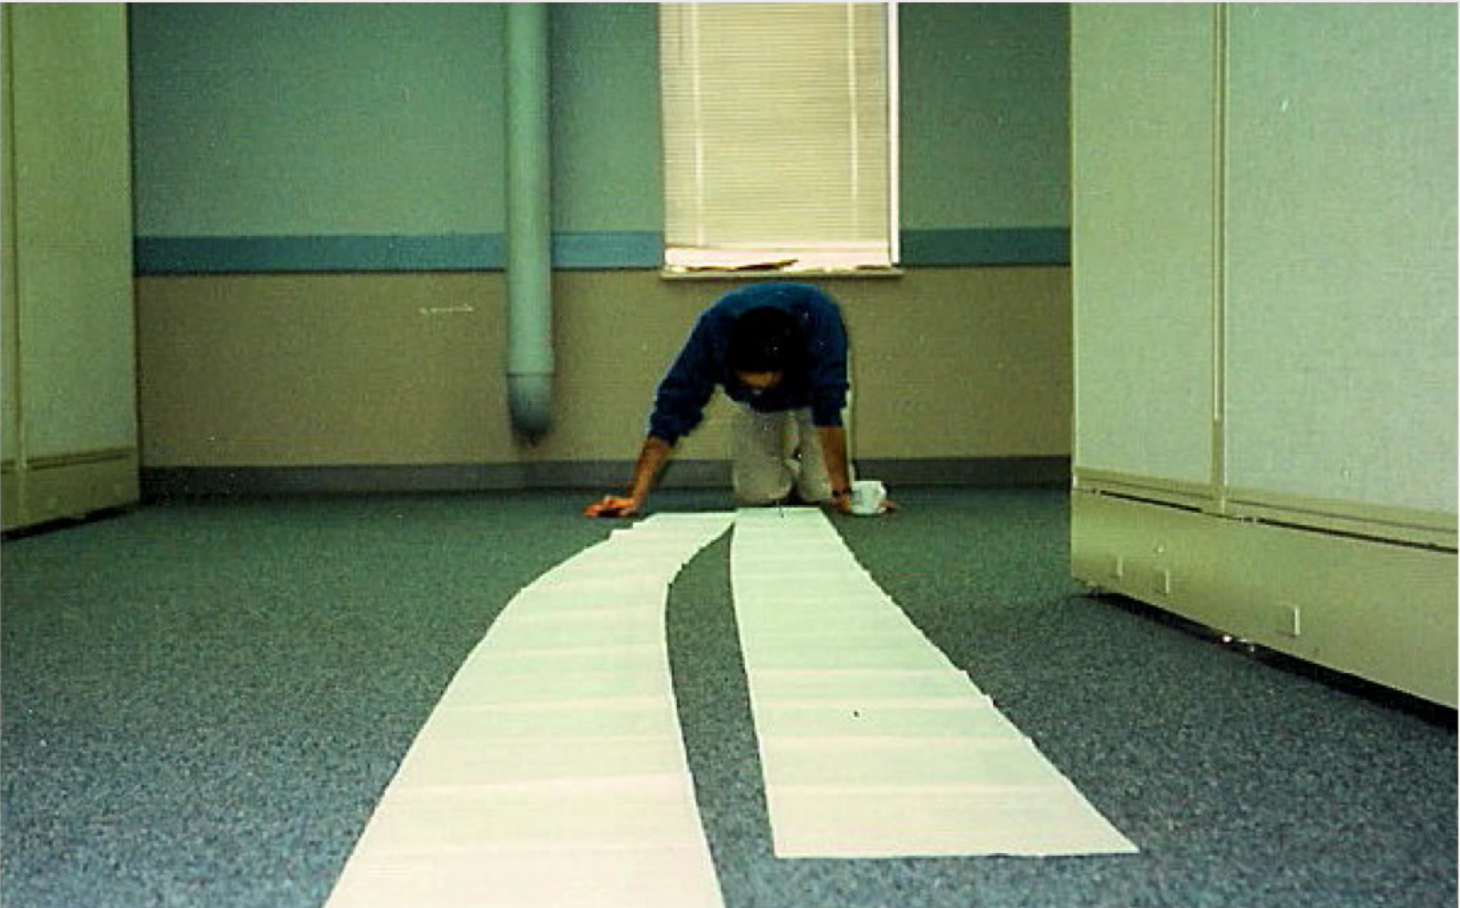
\includegraphics[scale=0.3]{old_code_review}
    \caption{https://www.youtube.com/watch?v=rHVlFOB5BpU}
  \end{figure}
\end{frame}

\begin{frame}
  \frametitle{Fases da Review}
  \begin{figure}[ht]
    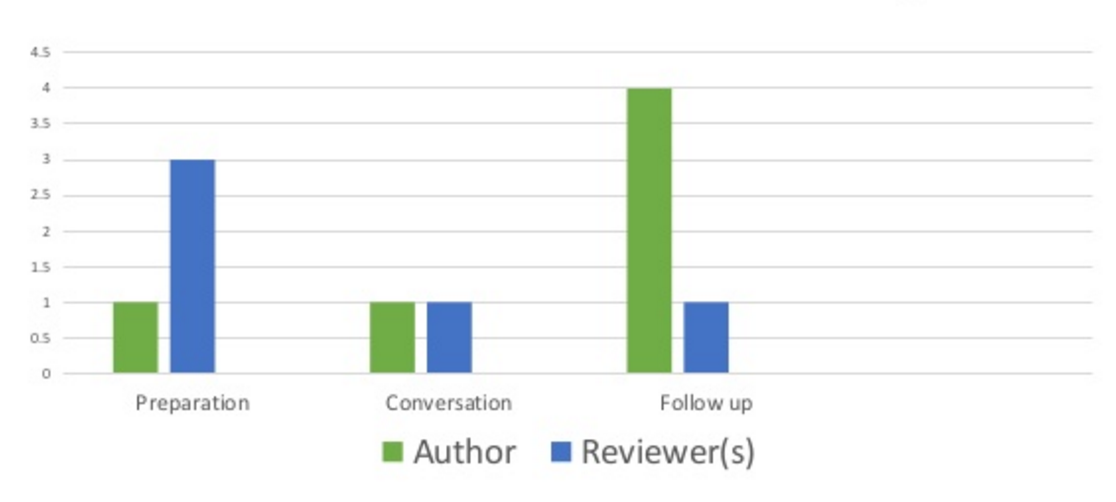
\includegraphics[scale=0.5]{not_a_meeting}
    \caption{http://www.slideshare.net/jprusakova/effective-codereview-color}
  \end{figure}
\end{frame}

\begin{frame}
  \frametitle{Limitade o tempo}
  \begin{figure}[ht]
    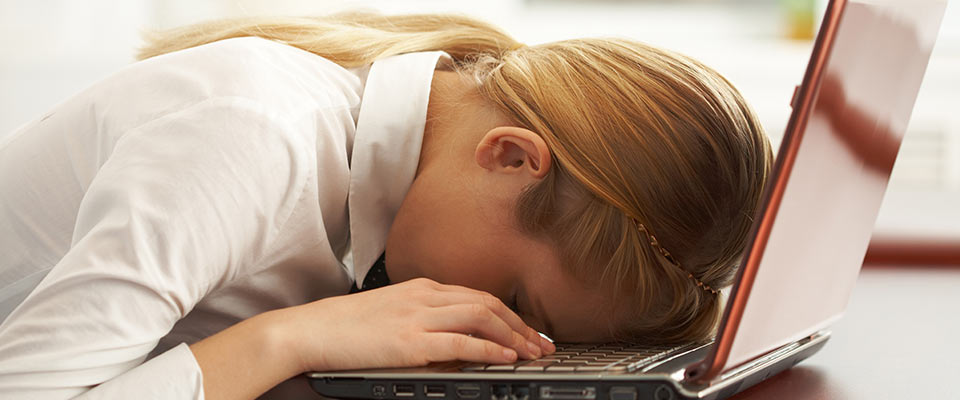
\includegraphics[scale=0.3]{tired}
    \caption{https://sites.psu.edu/siowfa14/2014/10/19/why-am-i-so-tired/}
  \end{figure}
\end{frame}

\begin{frame}
  \frametitle{Facede unha checklist}
  \begin{figure}[ht]
    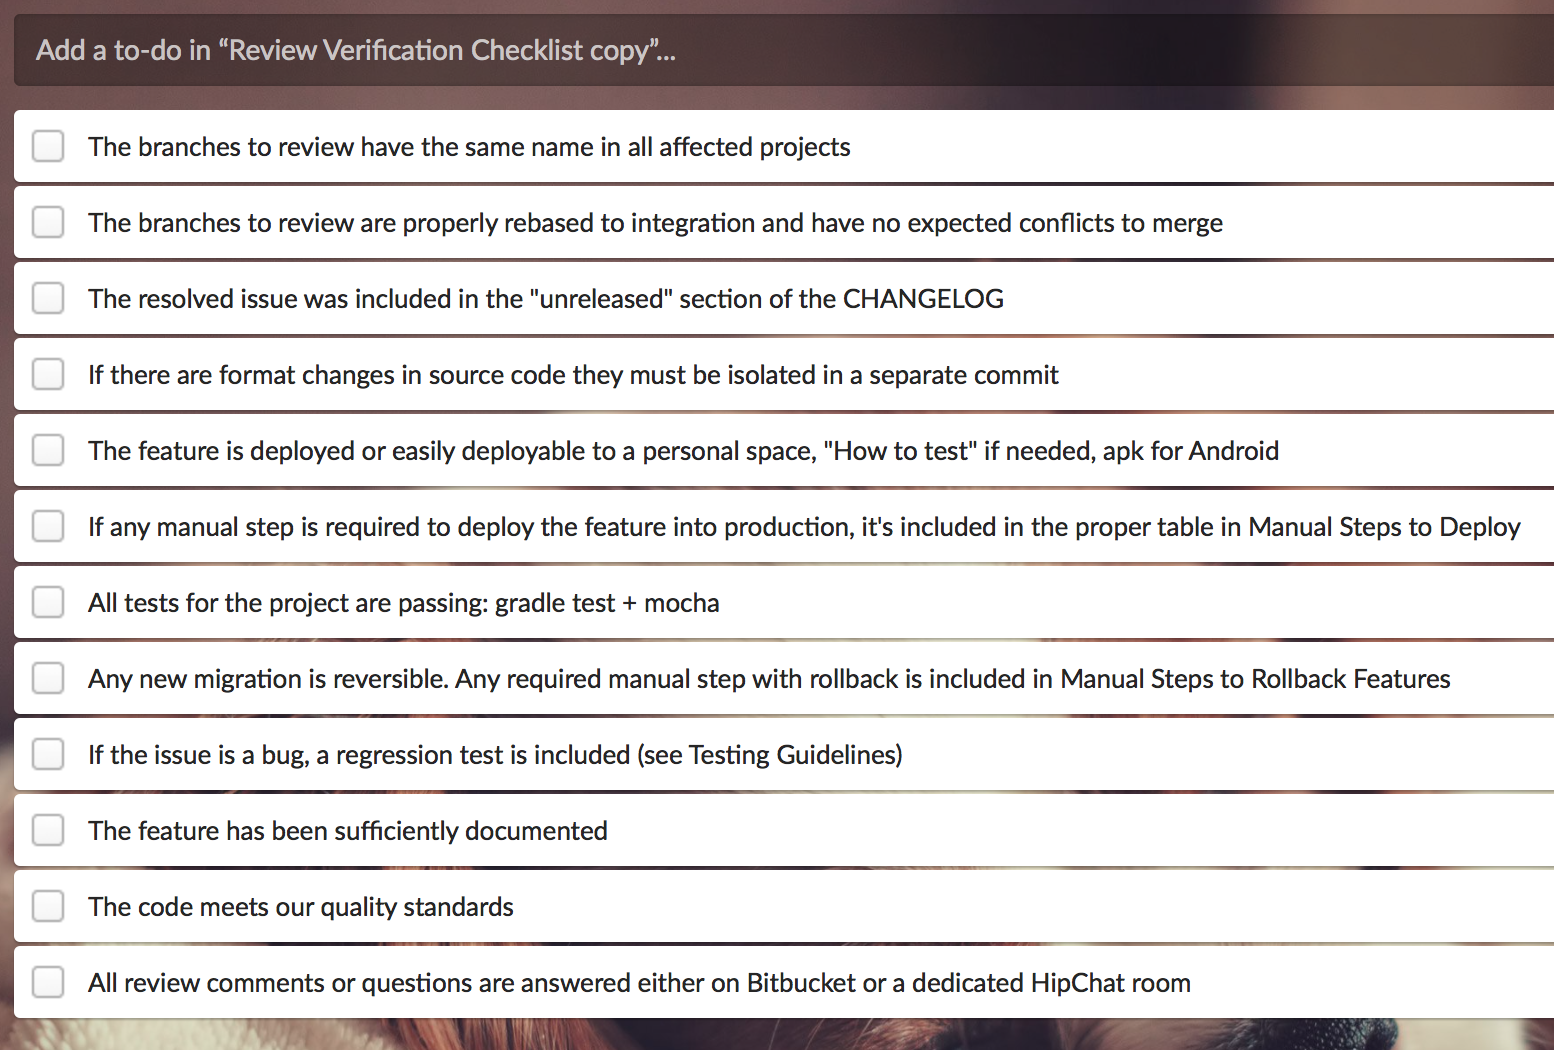
\includegraphics[scale=0.3]{review_checklist}
    \caption{My Review Checklist}
  \end{figure}
\end{frame}

\begin{frame}
  \frametitle{Medide}
  \begin{figure}[ht]
    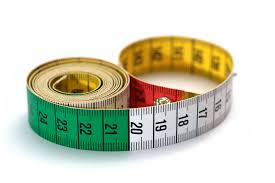
\includegraphics[scale=0.6]{metrics}
    \caption{Wikipedia}
  \end{figure}
\end{frame}

\begin{frame}
  \frametitle{Que midades!}
  \begin{figure}[ht]
    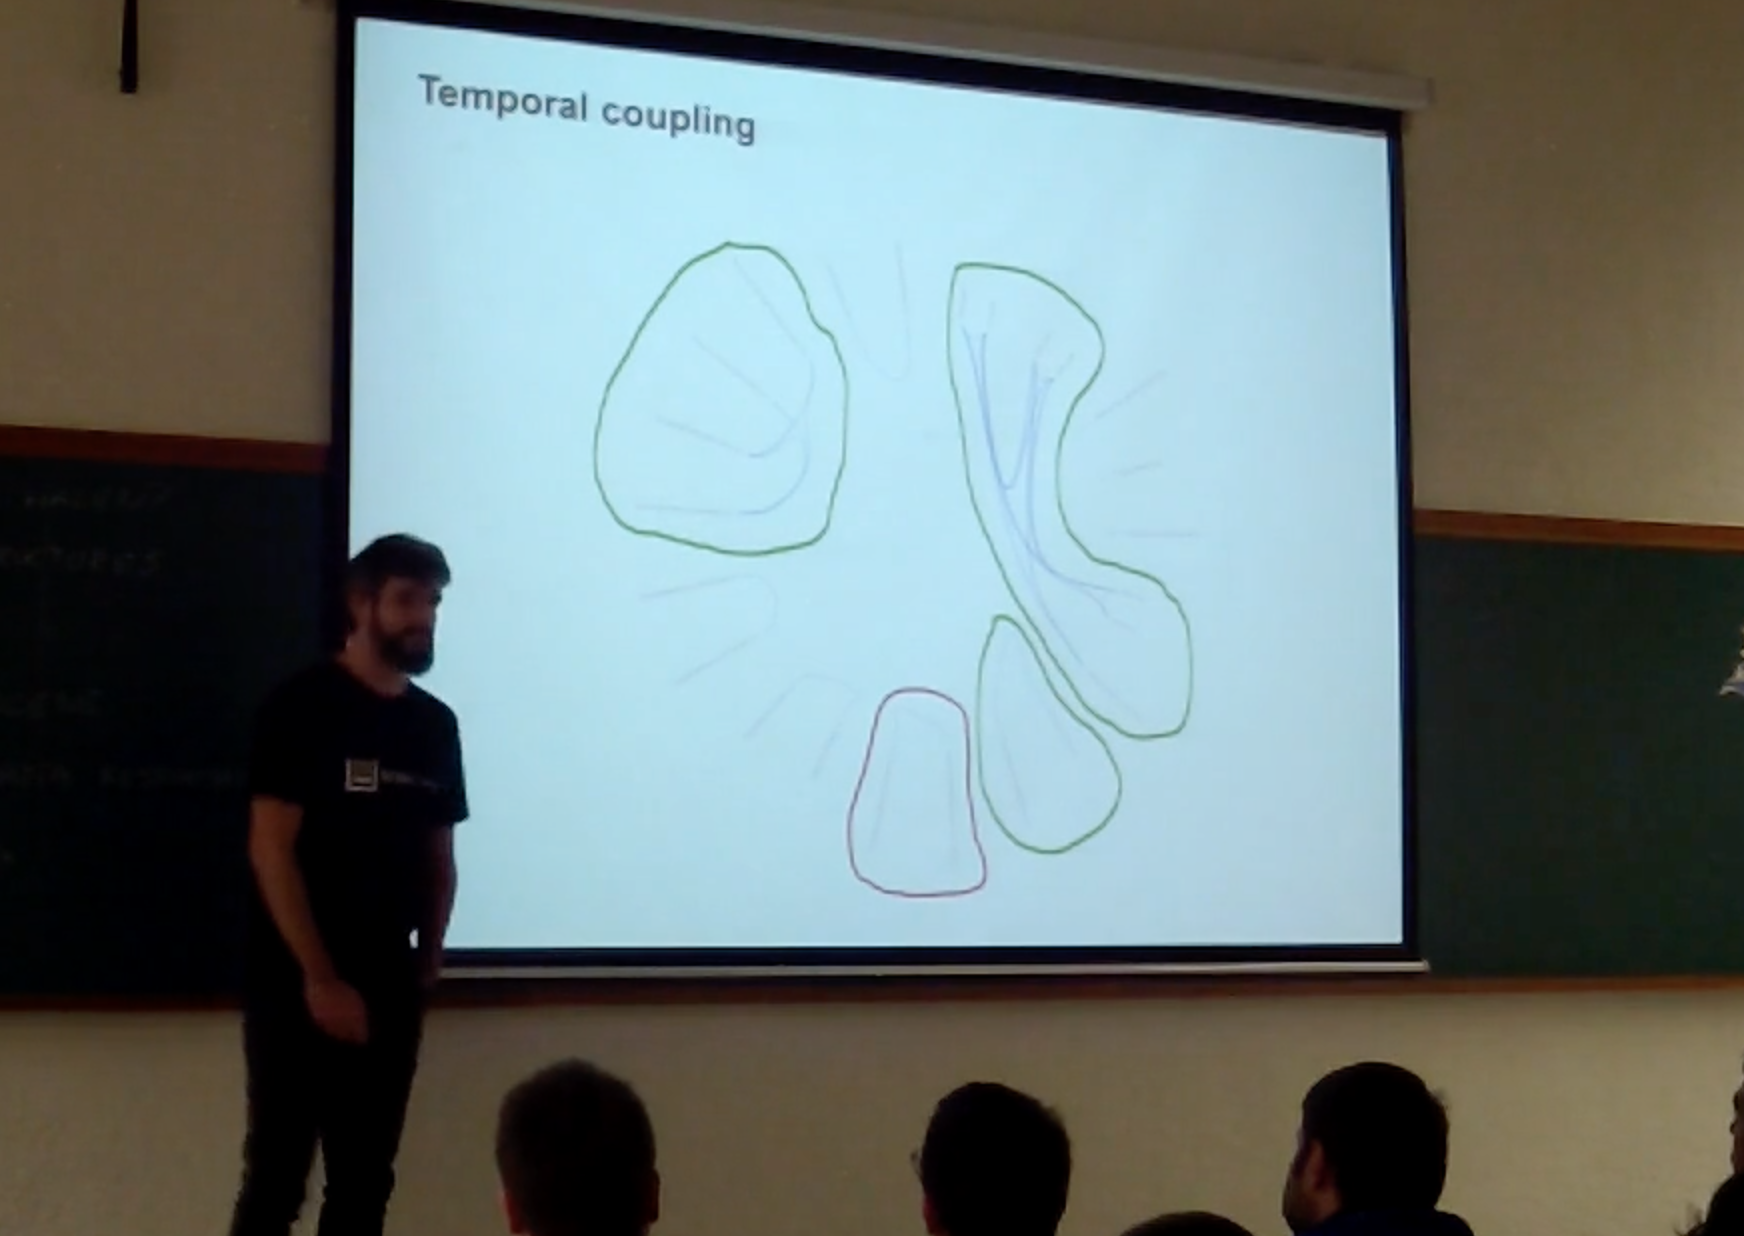
\includegraphics[scale=0.2]{vgaltes}
    \caption{Your Code as a Crime Scene - https://vimeo.com/154470784}
  \end{figure}
\end{frame}

\begin{frame}
  \frametitle{Medir é divertido, en serio}
  \begin{figure}[ht]
    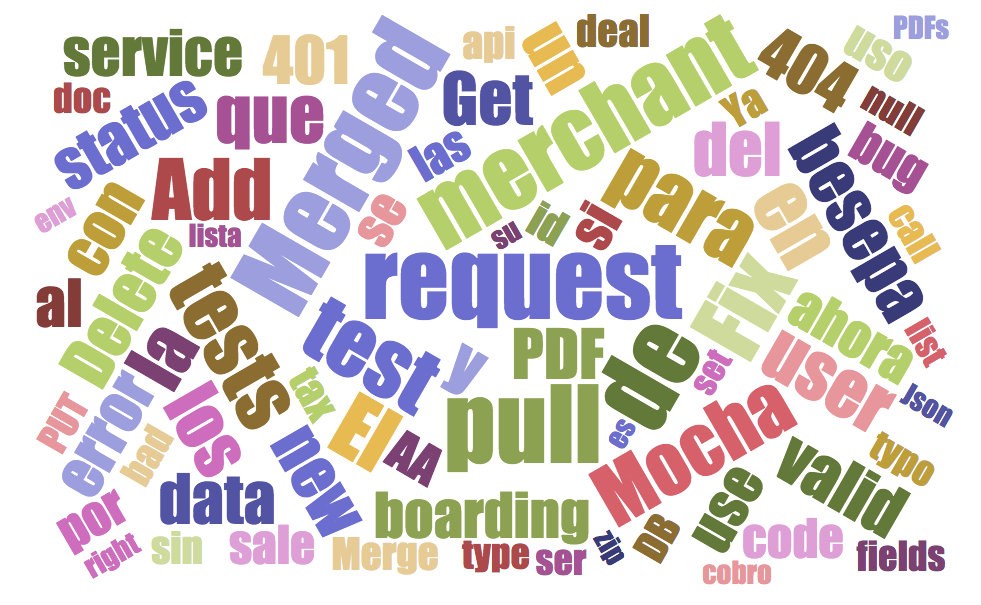
\includegraphics[scale=0.3]{tags}
  \end{figure}
\end{frame}

\begin{frame}
  \frametitle{Outra métrica sinxela}
  \begin{figure}[ht]
    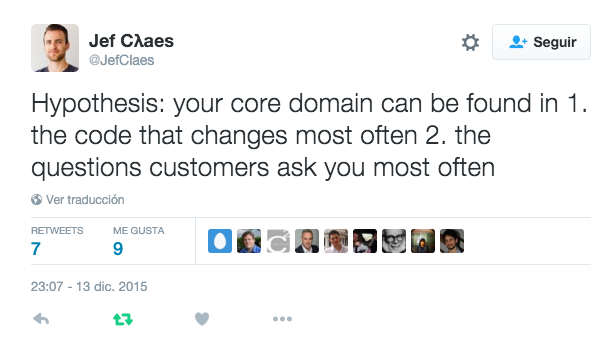
\includegraphics[scale=0.4]{your_domain}
  \end{figure}
\end{frame}

\begin{frame}
  \frametitle{Tips para reviewers}
  \begin{itemize}
    \item Limita o tempo
    \item Fai unha checklist
    \item Mide para decidir que abordar
  \end{itemize}
\end{frame}

\begin{frame}
  \frametitle{Fai pulls pequenas}
  \begin{figure}[ht]
    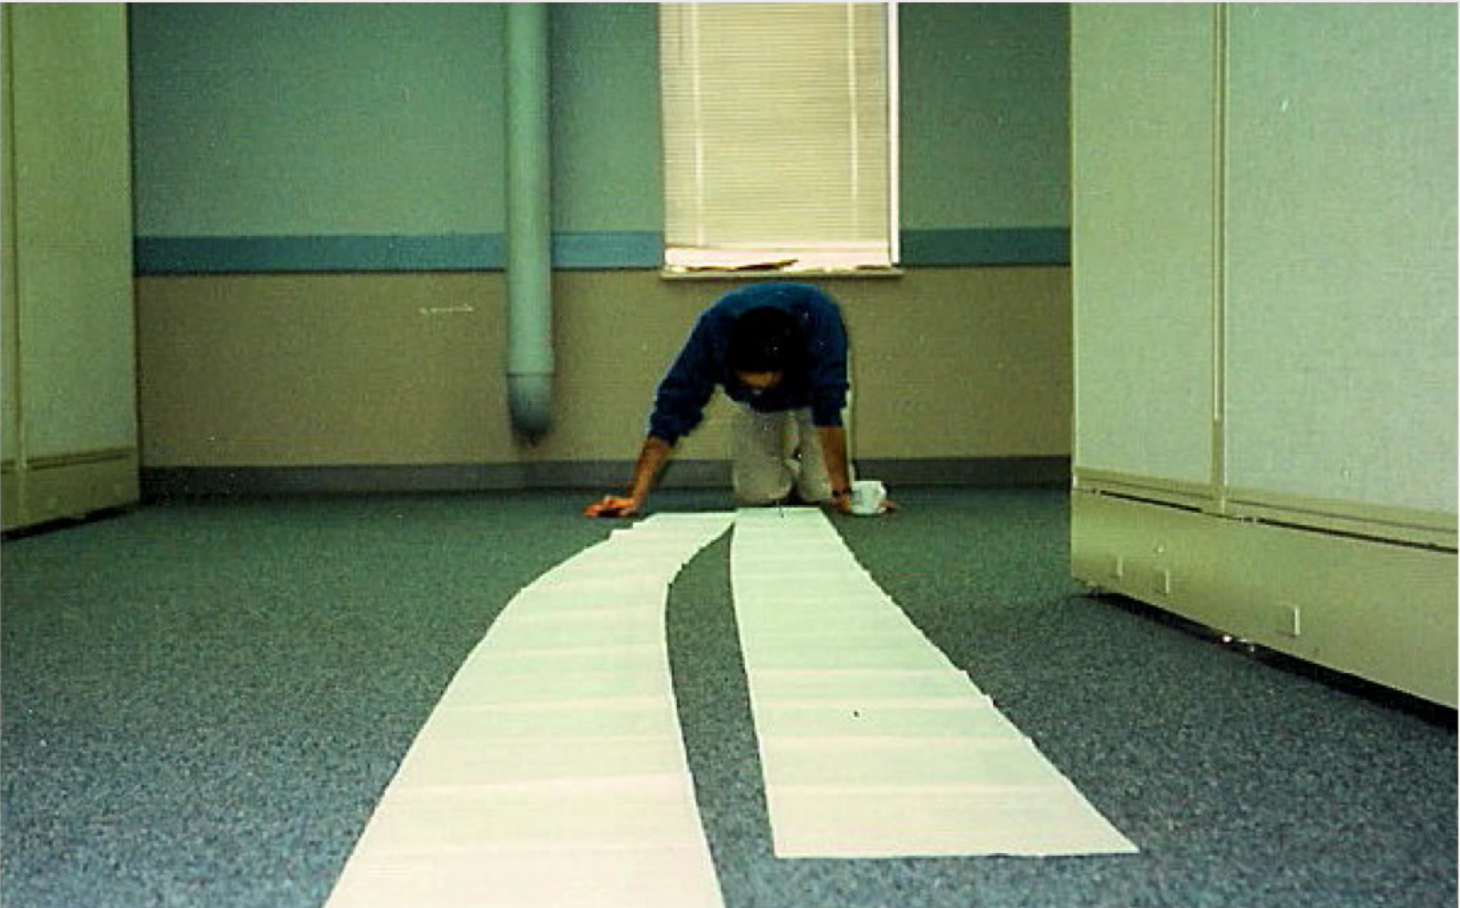
\includegraphics[scale=0.3]{old_code_review}
    \caption{https://www.youtube.com/watch?v=rHVlFOB5BpU}
  \end{figure}
\end{frame}

\begin{frame}
  \frametitle{Revisa ti antes}
  \begin{figure}[ht]
    \includegraphics[scale=0.2]{commit_push_run}
    \caption{https://www.reddit.com/r/ProgrammerHumor/comments/3nc531/in\_case\_of\_fire}
  \end{figure}
\end{frame}

\begin{frame}
  \frametitle{Automatiza}
  \begin{figure}[ht]
    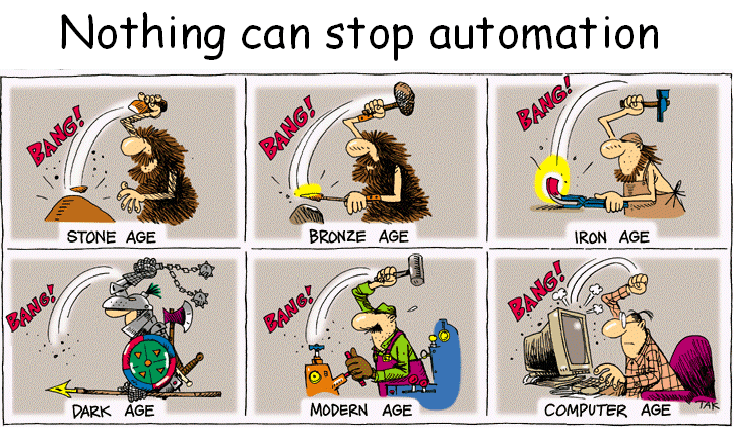
\includegraphics[scale=0.4]{automation}
    \caption{http://www.runmode.com/automationhumor.html}
  \end{figure}
\end{frame}

\begin{frame}
  \frametitle{Fai tests de regresión}
  \begin{figure}[ht]
    
\includegraphics[scale=0.3]{little_bugs}
    \caption{http://9gag.com/gag/a5dDw9o/99-little-bugs-in-the-code}
  \end{figure}
\end{frame}

\begin{frame}
  \frametitle{Tips para submitters}
  \begin{itemize}
    \item Fai pulls pequenas
    \item Revisa ti antes
    \item Automatiza
    \item Fai tests de regresión
  \end{itemize}
\end{frame}

\subsection{Como facer unha Code Review}
\label{subsec:Como}

\begin{frame}
  \frametitle{Big Brother vs Ego}
  \begin{figure}[ht]
    \centering
    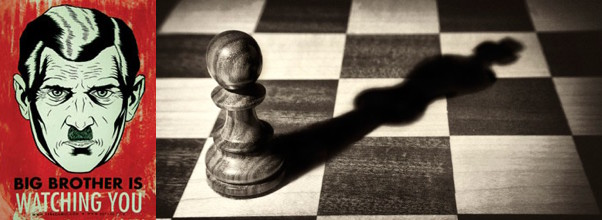
\includegraphics[scale=0.5]{ego}
    \caption{Wikipedia + http://www.sergerente.net/la-trampa-del-ego}
  \end{figure}
\end{frame}

\begin{frame}
  \frametitle{Acción vs visión}
  \blockquote{Vision without action is a dream. Action without vision is simply passing the time. Action with Vision is making a positive difference.}
  Joel Barker
\end{frame}

\begin{frame}
  \frametitle{Lei de Conway}
  \begin{figure}[ht]
    \centering
    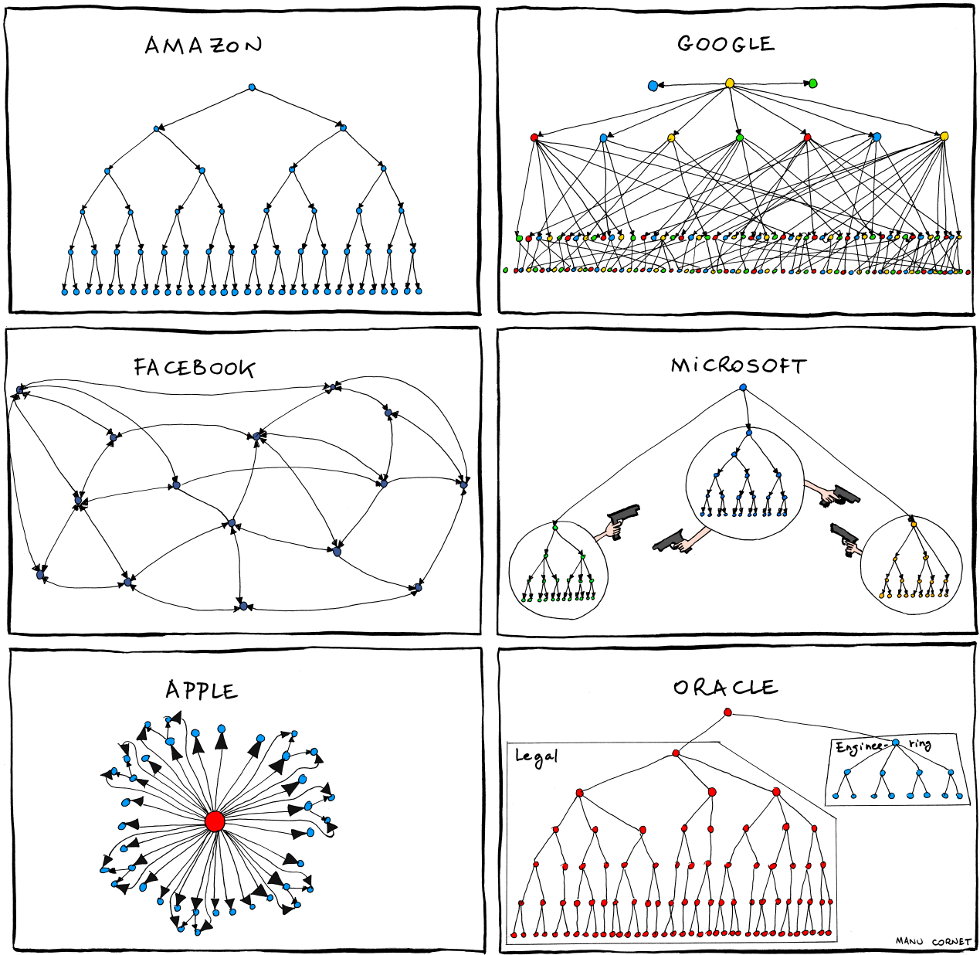
\includegraphics[scale=0.15]{conway}
    \caption{http://www.sixteensmallstones.org/conways-law-wiios-laws-software/}
  \end{figure}
\end{frame}

\begin{frame}
  \frametitle{Exceso de optimismo}
  \begin{figure}[ht]
    \centering
    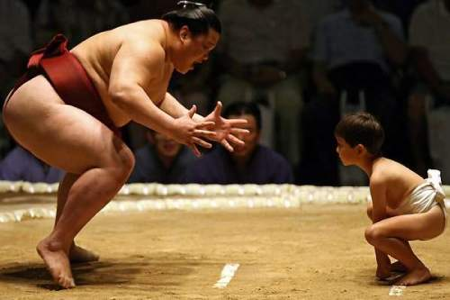
\includegraphics[scale=0.5]{optimism}
    \caption{https://mahifx.com/blog/aspects-of-behavioural-psychology-in-trading}
  \end{figure}
\end{frame}

\begin{frame}
  \frametitle{Lei de Parkinson da Trivialidade}
  \begin{figure}[ht]
    \centering
    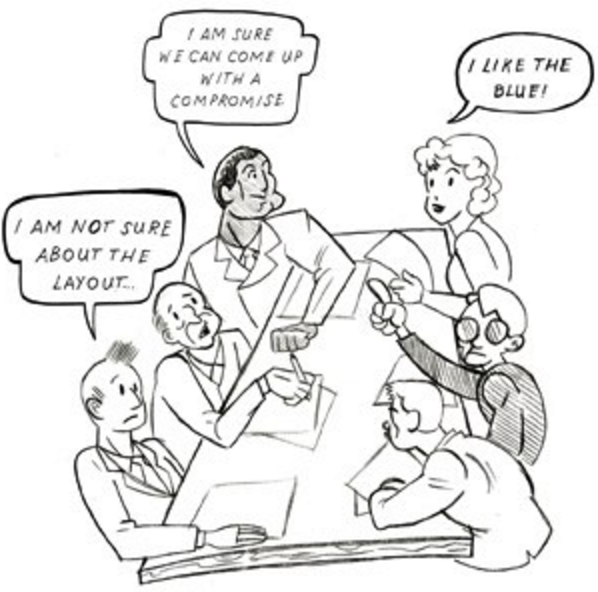
\includegraphics[scale=0.5]{triviality}
    \caption{http://www.zj86.cn/page/what-is-this\_net/fr/definition/triviality}
  \end{figure}
\end{frame}

\begin{frame}
  \frametitle{Tips}
  \begin{itemize}
    \item Chámase Code Review, non People Review
    \item Medide en vez de controlar
    \item Revisade todos
    \item Preguntade moito "por que"
    \item Discutide en persoa
    \item En lugar de ter razón, usade guías de estilo, métricas, ferramentas, ...
    \item Como submitter, ofrece contexto
    \item Como reviewer, pregunta alternativas
  \end{itemize}
\end{frame}

\begin{frame}
  \frametitle{Ideas para mellorar o código}
  \begin{itemize}
    \item Single Responsibility
    \item Open/Close
    \item Duplicación
    \item Eficiencia
    \item Manexo de erros
    \item Regra do boy scout
  \end{itemize}
\end{frame}

\begin{frame}
  \frametitle{Algúns malos olores}
  \begin{itemize}
    \item Nomes
    \item Lonxitudes
    \item Comentarios
    \item Número de parámetros
    \item Lexibilidade/estilo
  \end{itemize}
\end{frame}

\begin{frame}
  \frametitle{E o ingrediente segredo...}
  \begin{figure}[ht]
    \centering
    
\includegraphics[scale=0.15]{ingrediente_secreto}
    \caption{http://kungfupanda.wikia.com/}
  \end{figure}
\end{frame}
              % code reviews
% !TeX spellcheck = es_ES

% Funcionamento e uso de un CVS: Git
\title[Git Avanzado]{Git Avanzado}
\date{}
\author[Pepe Doval]{}
\institute{}

\section{Git Avanzado}
\label{sec:GitAvanzado}

\usebackgroundtemplate{%
  \tikz[overlay,remember picture] 
  \node[opacity=0.3 , at=(current page.south east),anchor=south east] {
    
\includegraphics[]{logo-labs}};
}

\begin{frame}
  \titlepage
  \begin{figure}[ht]
    \centering
    
\includegraphics[scale=0.2]{logo-git}
  \end{figure}
\end{frame}

\begin{frame}
  \frametitle{Táboa de contidos}
  \tableofcontents[currentsection]
\end{frame}


\subsection{Entendendo git}
\label{subsec:Entendendo}

\begin{frame}
  \frametitle{Git é complicado?}
  \begin{figure}[ht]
    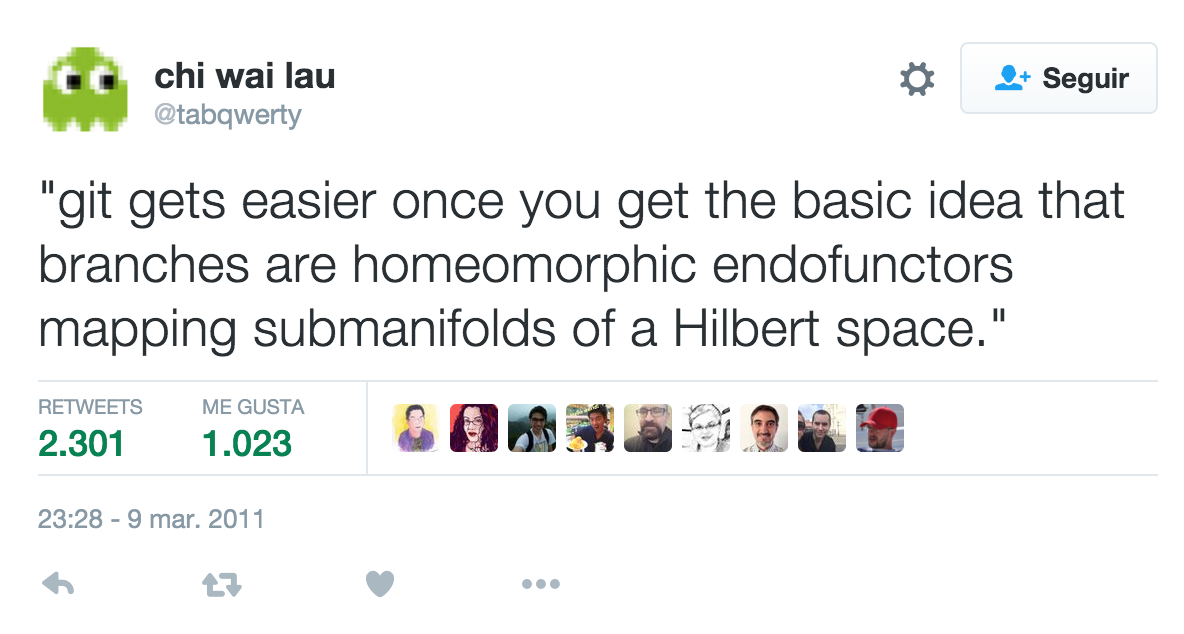
\includegraphics[scale=0.4]{git_not_hard}
    \caption{https://twitter.com/tabqwerty/status/45611899953491968}
  \end{figure}
\end{frame}

\begin{frame}
  \frametitle{Por que git é diferente?}
  \begin{itemize}
    \item Non é complicado, é potente
    \item Debedes desaprender Subversion (ou o que toque)
    \item Debedes decidir como contar a historia
  \end{itemize}
\end{frame}

\begin{frame}[fragile]
  \frametitle{man}
\begin{verbatim}
	man git

	man git-log

	man git-cherry-pick
\end{verbatim}
\end{frame}

\begin{frame}
  \frametitle{Conceptos esenciais}
  \begin{itemize}
    \item SHA-1
    \item Grafo Dirixido Acíclico
    \item Working Directory
    \item Staging Area (index)
  \end{itemize}
\end{frame}

\begin{frame}
  \frametitle{Vocabulario básico}
  \begin{itemize}
    \item Commit
    \item Punteiros: branches, tags, HEAD
    \item Checkout
    \item Fast forward
    \item Merge
    \item Rebase
    \item Conflicto
    \item Reset
  \end{itemize}
\end{frame}

\begin{frame}
  \frametitle{Isto ten que quedar claro}
  \begin{figure}[ht]
    \centering
    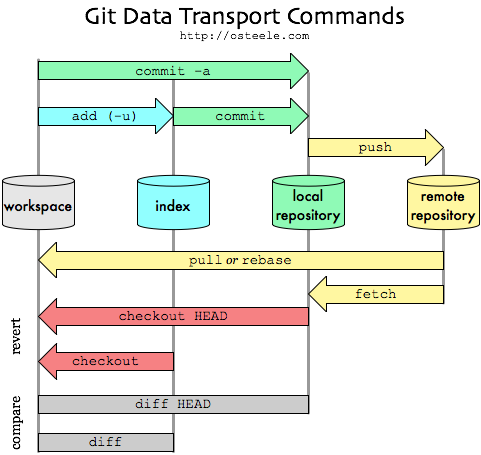
\includegraphics[scale=0.4]{flujo-git}
  \end{figure}
\end{frame}

\subsection{Construíndo a historia}
\label{subsec:Historia}

\begin{frame}[fragile]
  \frametitle{Para referenciar revisións e paths}
\begin{verbatim}
	git show 5f2df0d025026aa8785bde8cb32270aea3bac570
	git show 5f2df0d
	git show HEAD
	git show HEAD~1
	git show 5e75cda..ca1fc43
	git show :/Merged
	git checkout master
	git checkout master master
	git checkout -- master
	man git-rev-parse
\end{verbatim}
\end{frame}

\begin{frame}[fragile]
  \frametitle{Para preparar bos commits}
\begin{verbatim}
	git add -p
	git add -e
	git rm
	git mv
	git diff
	.gitignore
\end{verbatim}
\end{frame}

\begin{frame}[fragile]
  \frametitle{Para rescribir a historia}
\begin{verbatim}
	git commit --amend
	git stash
	git revert
	git cherry-pick
	git rebase -i
\end{verbatim}
\end{frame}

\begin{frame}[fragile]
  \frametitle{Para traballar en paralelo}
\begin{verbatim}
	git checkout -b mybranch master~1
	git format-patch 5e75cda..ca1fc43
	git apply 0001-Upgrade-version.patch
	git remote -v
	git remote add/rm
	git push/pull
	git init --bare
	git pull --rebase
	git push origin :master
\end{verbatim}
\end{frame}

\begin{frame}
  \frametitle{Que é e como facer unha pull request}
  \begin{figure}[ht]
    \centering
    
\includegraphics[scale=0.3]{pull_request}
    \caption{http://memegenerator.net/instance/62024625}
  \end{figure}
\end{frame}

\subsection{Utilidades para review}
\label{subsec:Review}

\begin{frame}[fragile]
  \frametitle{Para investigar na historia}
\begin{verbatim}
	git log --author=Pepe
	git log -Sconsole.log
	git blame de168bf9~1 README.md
	git bisect
\end{verbatim}
\end{frame}

\begin{frame}[fragile]
  \frametitle{Configuración avanzada}
\begin{verbatim}
	git config
	.gitconfig
	alias
\end{verbatim}
\end{frame}

\begin{frame}[fragile]
  \frametitle{Hooks}
\begin{verbatim}
	$ ls .git/hooks/

	applypatch-msg.sample     pre-push.sample
	commit-msg.sample         pre-rebase.sample
	post-update.sample        prepare-commit-msg.sample
	pre-applypatch.sample     update.sample
	pre-commit.sample
\end{verbatim}
\end{frame}

\begin{frame}
  \frametitle{Un dos grandes problemas da humanidade resolto!}
  \begin{figure}[ht]
    \centering
    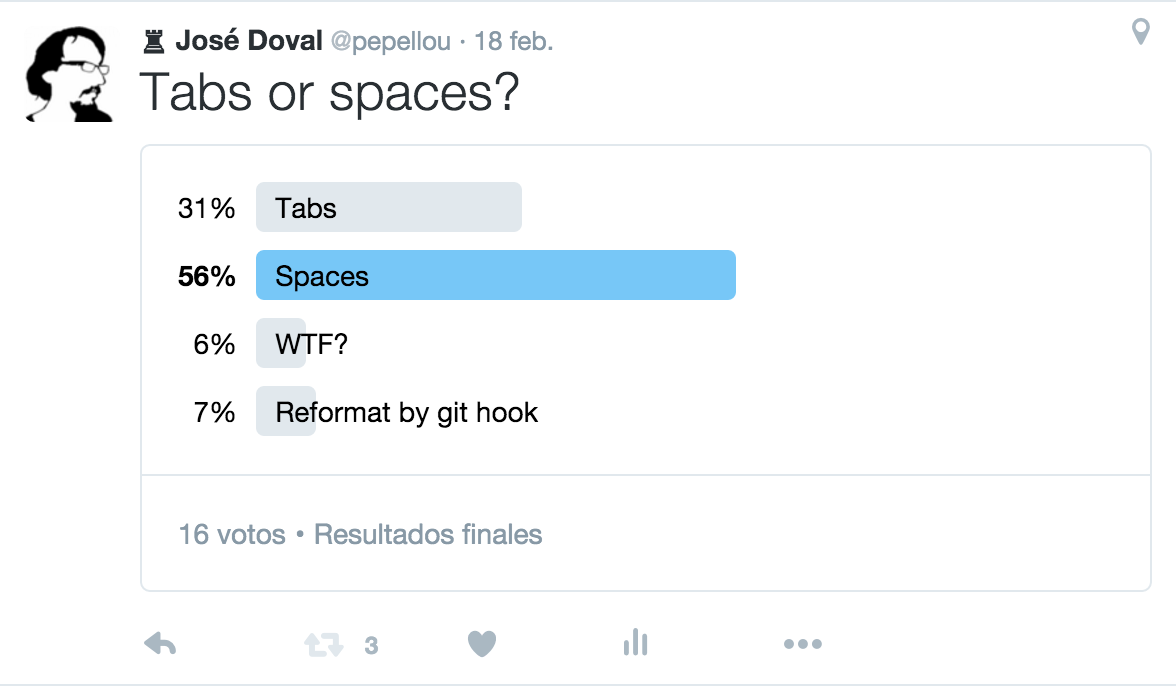
\includegraphics[scale=0.4]{tabs_vs_spaces}
  \end{figure}
\end{frame}

\subsection{Boas prácticas}
\label{subsec:BoasPracticas}

\begin{frame}
  \frametitle{Boas prácticas}
  \begin{itemize}
    \item Commits atómicos
    \item Commits frecuentes
    \item Non commitear traballo a medias
    \item Pasa os tests antes de commitear
    \item Escribe boas mensaxes de commit
    \item Usa branches, son gratis
    \item Usade todos o mesmo workflow no equipo
  \end{itemize}
\end{frame}

\begin{frame}
  \frametitle{Dúbidas?}
  \begin{figure}[ht]
    \centering
    
\includegraphics[scale=0.3]{dubidas}
    \caption{http://memegenerator.net/instance/62024625}
  \end{figure}
\end{frame}

              % git avanzado

\end{document}
